\documentclass[12pt,a4paper]{article}
\usepackage[polish]{babel}
\usepackage[utf8]{inputenc}
\usepackage{graphicx}
\usepackage{float}
\usepackage{listings}
\usepackage{caption}
\usepackage{geometry}
\geometry{margin=2.5cm}

\title{Algorytmy i struktury danych lista 1}
\author{Bartosz Polak}
\date{27.10.2025}

\lstset{
  basicstyle=\ttfamily\small,
  numbers=left,
  numberstyle=\tiny,
  frame=single,
  breaklines=true,
  postbreak=\mbox{\textcolor{red}{$\hookrightarrow$}\space},
  captionpos=b
}

\begin{document}
\maketitle

\section{Wprowadzenie}
Celem listy jest analiza oraz porównanie efektywności różnych algorytmów sortowania zaimplementowanych w ~C++. 
Mierzone były:
\begin{itemize}
  \item liczba porównań elementów,
  \item liczba przypisań elementów.
\end{itemize}
Dla każdego algorytmu przeprowadzono testy na tablicach o różnych rozmiarach, a wyniki zestawiono w tabelach oraz na wykresach.

\section{Analizowane algorytmy}
\begin{itemize}
  \item \textbf{Insertion Sort} oraz jego modyfikacja polegająca na wstawianiu "na raz" dwóch elementó tablicy,
  \item \textbf{Merge Sort} 2-dzielny i 3-dzielny,
  \item \textbf{Heap Sort} binarny i ternarny.
\end{itemize}

\section{Najciekawsze fragmenty kodu}

\subsection{Algorytm sortowania przez wstawianie}
Poniżej przedstawiono fragment klasycznego algorytmu sortowania przez wstawianie wraz z liczeniem operacji:
\begin{lstlisting}[language=C++,caption={Fragment funkcji INSERTION\_SORT}]
for (int i = 1; i < n; i++) {
    x = A[i];
    przypisania++;
    j = i - 1;
    przypisania++;
    while (true) {
        porownania++;
        if (j < 0) break;
        porownania++;
        if (A[j] > x) {
            A[j + 1] = A[j];
            przypisania++;
            j--;
            przypisania++;
        } else break;
    }
    A[j + 1] = x;
    przypisania++;
}
\end{lstlisting}

Druga wersja, \texttt{INSERTION\_SORT2}, wprowadza jednoczesne wstawianie dwóch elementów, co potencjalnie mogłoby redukować liczbę porównań i przypisań.

\subsection{Sortowanie przez scalanie 2-dzielne i 3-dzielne}
Fragment implementacji funkcji scalającej dla sortowania 3-dzielnego:
\begin{lstlisting}[language=C++,caption={Fragment funkcji MERGE3}]
while (i < n1 || j < n2 || m < n3) {
    int min_val = 1000000000;
    int min_index = 0;
    if (i < n1 && L1[i] < min_val) { min_val = L1[i]; min_index = 1; }
    if (j < n2 && L2[j] < min_val) { min_val = L2[j]; min_index = 2; }
    if (m < n3 && L3[m] < min_val) { min_val = L3[m]; min_index = 3; }
    if (min_index == 1) A[r++] = L1[i++];
    else if (min_index == 2) A[r++] = L2[j++];
    else if (min_index == 3) A[r++] = L3[m++];
}
\end{lstlisting}
Algorytm 3-dzielny cechuje się większą złożonością implementacyjną, ale w praktyce może lepiej równoważyć rekurencję. Aby zmodyfikować merge sort 2-dzielny do 3-dzielnego bez skomplikowanego zagnieżdżania "if", musiałem wprowadzić zmienne min\_val i min\_index, co jest ciekawym rozwiązaniem problemu.

\subsection{Sortowanie przez kopcowanie binarne i trójkowe}
Porównano wersję klasyczną kopca binarnego z wersją kopca trójkowego:
\begin{lstlisting}[language=C++,caption={Fragment funkcji heapify\_ternary}]
int largest = i;
int c1 = 3 * i + 1;
int c2 = 3 * i + 2;
int c3 = 3 * i + 3;

if (c1 < n && A[c1] > A[largest]) largest = c1;
if (c2 < n && A[c2] > A[largest]) largest = c2;
if (c3 < n && A[c3] > A[largest]) largest = c3;

if (largest != i) {
    swap(A[i], A[largest]);
    przypisania += 3;
    heapify_ternary(A, n, largest, porownania, przypisania);
}
\end{lstlisting}

\section{Porównanie wyników działania algorytmów}

Dla różnych rozmiarów tablic ($n = 10, 100, 1000, 5000, 10000$) zmierzono liczbę porównań i przypisań.  
Poniżej przedstawiono zestawienie wyników w postaci wykresów.

\begin{figure}[H]
    \centering
    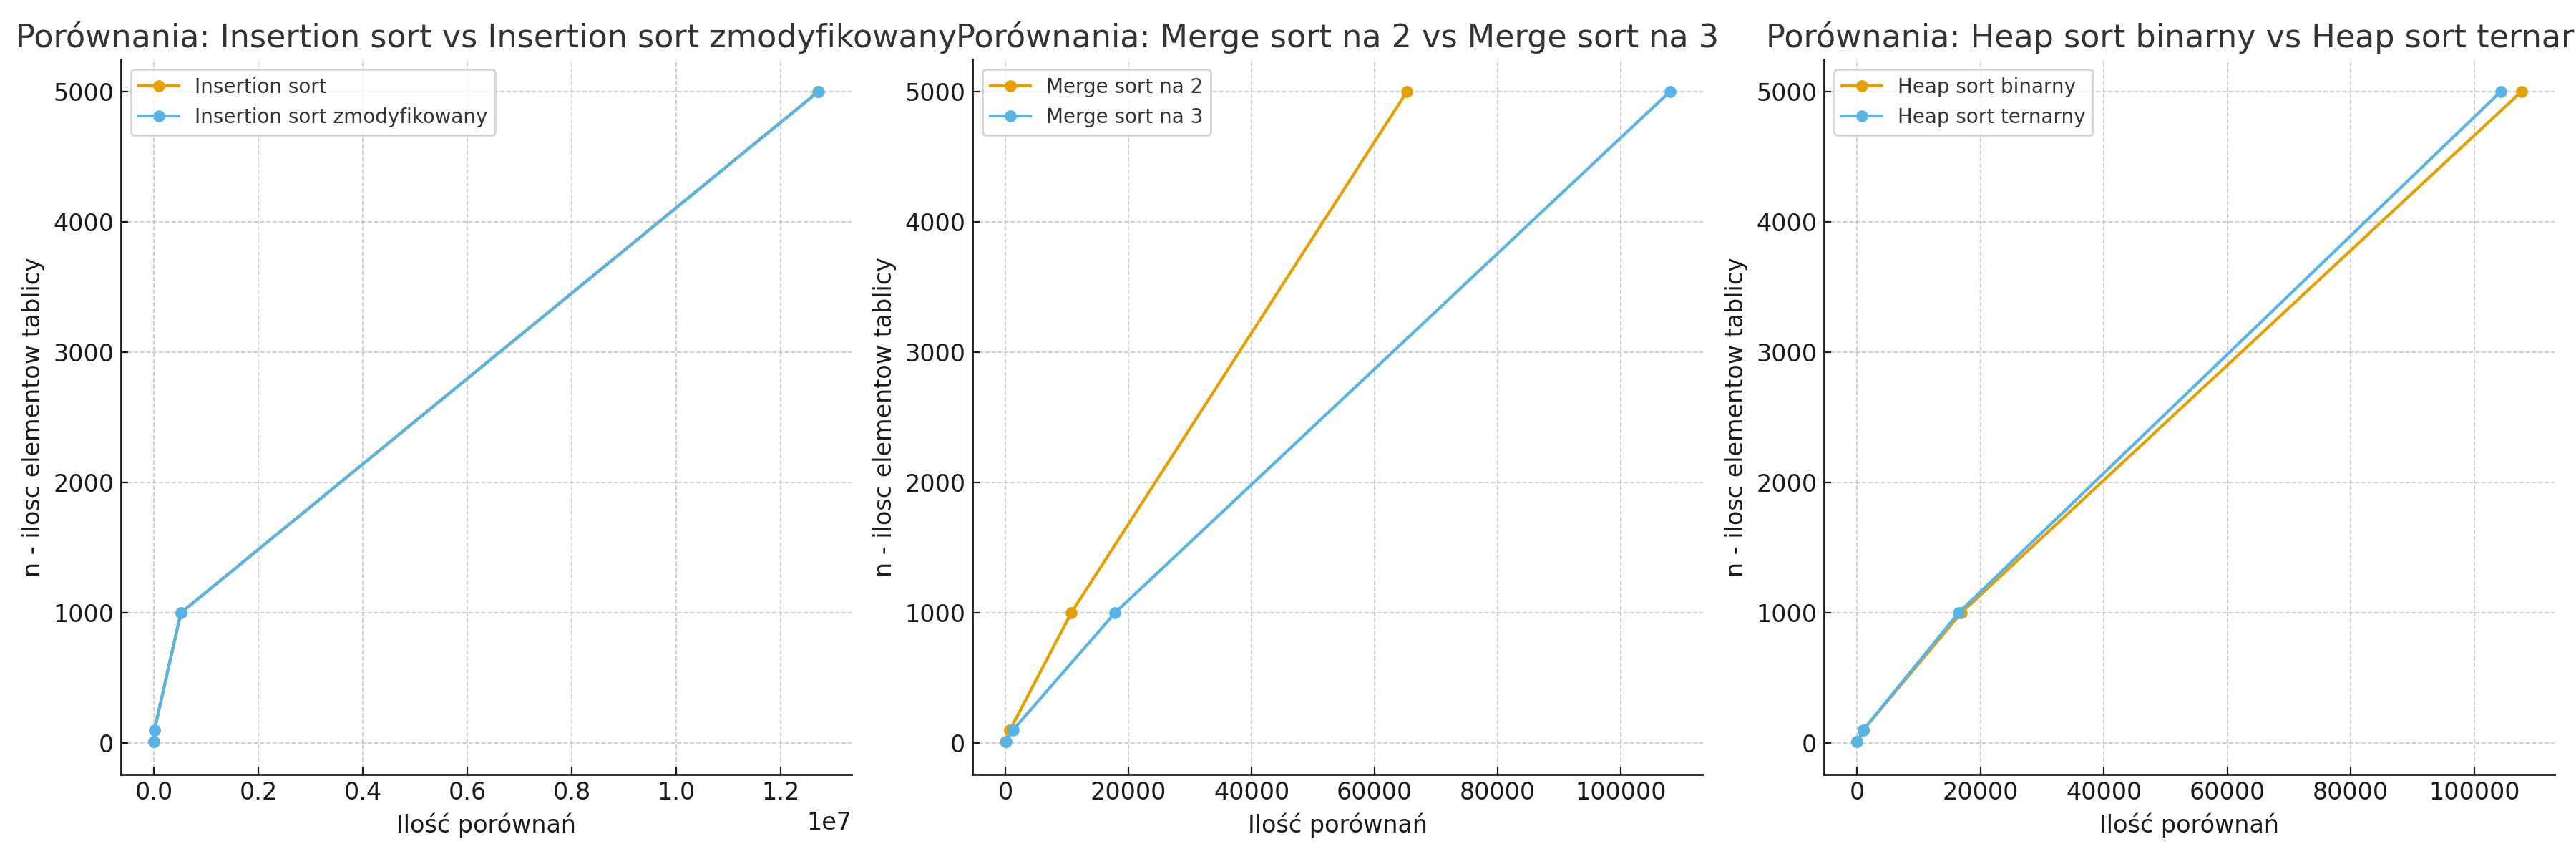
\includegraphics[width=0.9\linewidth]{wykresy_porownania.png}
    \caption{Porównanie liczby porównań dla różnych algorytmów.}
\end{figure}

\begin{figure}[H]
    \centering
    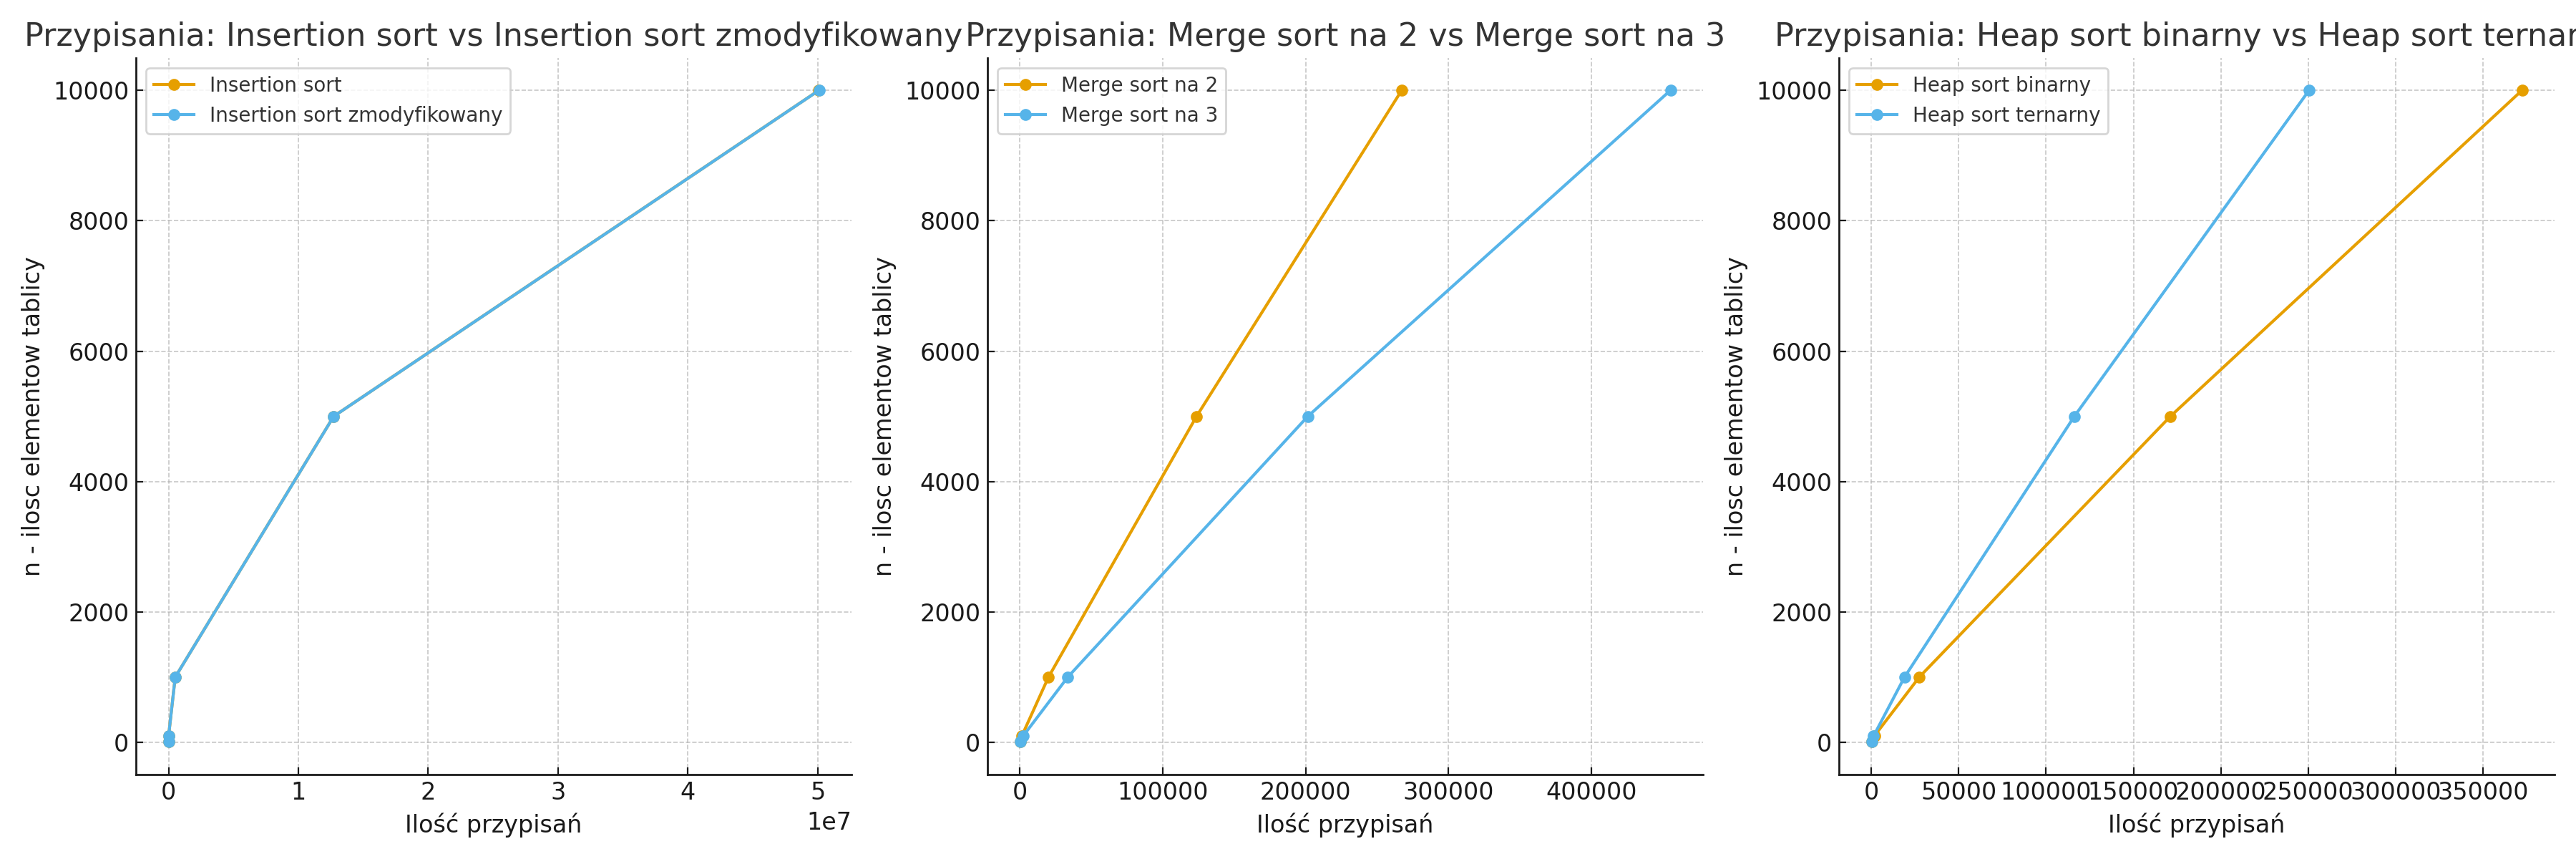
\includegraphics[width=0.9\linewidth]{wykresy_przypisania.png}
    \caption{Porównanie liczby przypisań dla różnych algorytmów.}
\end{figure}

\section{Wnioski}
\begin{itemize}
  \item Klasyczny \textbf{Insertion Sort} jest najmniej efektywny dla dużych zbiorów danych, jego złożoność $O(n^2)$ powoduje gwałtowny wzrost liczby operacji.
  \item Modyfikacja \textbf{Insertion Sort} przynosi nieznaczącą różnicę, niezauważalną na wykresie.
  \item \textbf{Merge Sort 3-dzielny} generuje więcej operacji przypisań i porównań niż klasyczny Merge Sort 2-dzielny.
  \item \textbf{Heap Sort} binarny oraz trójkowy mają porównywalne wyniki w ilości porównań, gdzie wersja binarna wykonuje mało znacząco mniej przypisań, ale też bardziej znacząco więcej przypisań.
  \item Dla dużych danych najlepsze rezultaty osiągały algorytmy o złożoności $O(n \log n)$ – \textbf{Merge Sort} oraz \textbf{Heap Sort}.
\end{itemize}

\section{Podsumowanie}
Wszystkie zaimplementowane algorytmy poprawnie sortują dane wejściowe, jednak różnią się efektywnością.  
Z punktu widzenia praktycznego — dla dużych tablic — najbardziej opłacalne są algorytmy typu \textbf{Merge Sort} i \textbf{Heap Sort}, natomiast \textbf{Insertion Sort} pozostaje użyteczny jedynie dla bardzo małych zbiorów.

\end{document}
